% Created 2017-01-29 Sun 12:47
% Intended LaTeX compiler: pdflatex
\documentclass[presentation]{beamer}
\usepackage[utf8]{inputenc}
\usepackage[T1]{fontenc}
\usepackage{graphicx}
\usepackage{grffile}
\usepackage{longtable}
\usepackage{wrapfig}
\usepackage{rotating}
\usepackage[normalem]{ulem}
\usepackage{amsmath}
\usepackage{textcomp}
\usepackage{amssymb}
\usepackage{capt-of}
\usepackage{hyperref}
\usepackage[version=3]{mhchem}
\usepackage{minted}
\usetheme{Madrid}
\author{Willian Paiva \& Nathalie Craeye}
\date{\today}
\title{Context-Oriented Programming}
\hypersetup{
 pdfauthor={Willian Paiva \& Nathalie Craeye},
 pdftitle={Context-Oriented Programming},
 pdfkeywords={},
 pdfsubject={},
 pdfcreator={Emacs 25.1.1 (Org mode 9.0.4)}, 
 pdflang={English}}
\begin{document}

\maketitle
\begin{frame}{Outline}
\tableofcontents
\end{frame}


\section{Introduction to Context-Oriented Programming}
\label{sec:org203da34}

\begin{frame}[label={sec:org06c2a92}]{The objective}
\begin{block}{Simplification and control}
\begin{itemize}
\item Make it simpler to take the context in consideration.
\item Better control over the method selection.
\item Well define the entities.
\item Tackle \emph{crosscutting-concerns}.
\end{itemize}
\end{block}
\end{frame}



\begin{frame}[label={sec:org1fee1dc}]{Context and behavior variants}
COP subdivides the Context into 3 categories:
\begin{block}{Actor}
Ex: Function or methods call, messages \ldots{}
\end{block}
\begin{block}{Environment}
Ex: GPS, battery, light sensor \ldots{} 
\end{block}
\begin{block}{System}
Ex: Methods, objects, subsystems \ldots{}
\end{block}
\end{frame}


\begin{frame}[label={sec:orgd6e65b4}]{Multi-dimensional message dispatch}
\begin{block}{one dimension (Procedural programming)}
\begin{center}
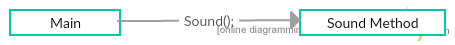
\includegraphics[width=.9\linewidth]{./one.jpg}
\end{center}
\end{block}
\end{frame}

\begin{frame}[label={sec:orge354381}]{Multi-dimensional message dispatch}
\begin{block}{two dimension (Object-oriented programming)}
\begin{center}
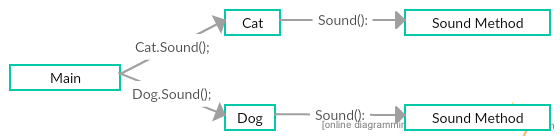
\includegraphics[width=.9\linewidth]{./two.png}
\end{center}
\end{block}
\end{frame}


\begin{frame}[label={sec:org58f7b3a}]{Multi-dimensional message dispatch}
\begin{block}{three dimension (Subject-oriented programming)}
\begin{center}
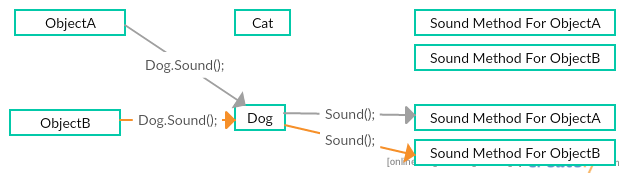
\includegraphics[width=.9\linewidth]{./three.png}
\end{center}
\end{block}
\end{frame}


\begin{frame}[label={sec:org8d86638}]{Layers}
\begin{block}{Definitions}
\begin{itemize}
\item First-class entities
\item Activation and deactivation
\begin{itemize}
\item Arbitrary parts of the code
\item Conditional (environment)
\end{itemize}
\item Scope
\begin{itemize}
\item executes the code on the scope in or out the layer
\end{itemize}
\end{itemize}
\end{block}
\end{frame}

\begin{frame}[fragile,label={sec:orgc7dcc58}]{Multi-dimensional message dispatch}
 \begin{block}{four dimension (Context-oriented programming)}
\begin{minted}[frame=lines,fontsize=\scriptsize]{java}
class Calculate{
    Calculate(){};
    Void HeavyCalc(){ someHeavyCalc();}
    Layer batWarning {
        void HeavyCalc(){
            sendNotification(" Warning Low Battery level");
            proceed();
        }
    }
    Layer lowMemory {
        void HeavyCalc(){
            sendNotification("Not enough memory to execute");
            throw new NotEnoughtMemoryException();
        }
    }
}
\end{minted}
\end{block}
\end{frame}


\begin{frame}[fragile,label={sec:org7496f79}]{Multi-dimensional message dispatch}
 \begin{block}{four dimension  cont\ldots{}}
\begin{minted}[frame=lines,fontsize=\scriptsize]{java}
Calculate c = new Calculate();
if(SystemMemory() < mimMem){
    with(lowMemory){
        c.HeavyCalc();
    }
}else if(BatteryLevel() < mimBat){
    with(batWarning){
        c.HeavyCalc();
    }
}else{
    c.HeavyCalc();
}
\end{minted}
\end{block}
\end{frame}

\section{Related Solutions}
\label{sec:orge928c76}

\begin{frame}[label={sec:org55587d9}]{Decorator pattern}
\begin{block}{Common intents}
\begin{itemize}
\item Can withdrawn responsibilities.(???)
\item Add behavior or state to individual objects at run-time.
\end{itemize}
\end{block}

\begin{block}{Cons}
\begin{itemize}
\item With COP it is possible to activate and deactivate layers with a simpler syntax.
\end{itemize}
\end{block}

\begin{block}{Pros}
\begin{itemize}
\item By using the decorator pattern a class don't need to know/declare future \emph{"decorations"}.
\end{itemize}
\end{block}
\end{frame}



\begin{frame}[label={sec:orgf60373f}]{Aspect-oriented programming}
\begin{block}{Advantages over COP}
\begin{itemize}
\item Decrease code scattering by a static way of programming.
\item The class has no knowledge of the aspects.
\item Provides similar functionalities with (\emph{pointcut}, \emph{after} and \emph{before}).
\item Integrated in many more languages like Java and C++.
\end{itemize}
\end{block}
\end{frame}

\begin{frame}[label={sec:org2e4cac1}]{Q\&A}
\begin{center}

\includegraphics[width=.9\linewidth]{./qa.jpg}
\end{center} 
\end{frame}
\end{document}